\newpage

\section{Canvas}
O Project Model Canvas é um quadro auxiliar no processo de gerenciamento de projetos, o qual nele consta justificativas, stakeholders, equipe, produto, objetivos entre outros. 

\subsection{Justificativas}
\par Altos Gastos Energéticos: A faculdade do Gama (FGA) tem um consumo de energia elevado devido a utilização de equipamentos de alta potência, encontrados em laboratórios, salas de aulas, salas de professores, nas dependências gerais e no Restaurante Universitário (RU). Esses gastos elevados de energia elétrica podem ser comprovados com as contas de energia elétrica da FGA.
\par Perdas e ineficiência de transmissões: A falta de manutenção nas instalações elétricas e equipamentos é um fator que contribui para o elevado custo com eletricidade da FGA, pois esta situação provoca uma redução no rendimento dos equipamentos e da distribuição de energia. Um exemplo dessa situação são os projetores das salas superiores do EAD, que devido à falta de manutenção as imagens projetadas acabam ficando com pouca qualidade, além das instalações dos laboratórios de informática onde há fios expostos.
\par Utilização de Fontes Tradicionais de Energia Elétrica: As Fontes tradicionais no cenário brasileiro são as hidrelétricas, que podem ter oscilações sazonais de produção por fatores climáticos, o que pode interferir na estabilidade do serviço e no preço.
\par Dependência da Companhia de Eletricidade de Brasília (CEB): A dependência da companhia pode gerar uma série de fatores desagradáveis, como burocracia para resolver problemas simples que trazem deficiência ao fornecimento da eletricidade, além dos custos com a mudança de tarifas de energia elétrica como a bandeira vermelha.

\subsection{Objetivos Smart Grid}
Projetar um sistema Smart Grid para a FGA interligado as duas fontes renováveis em um período de um trimestre.

\subsection{Benefícios futuros}
Incentivo ao uso de fontes renováveis: O projeto propõe a utilização de fontes renováveis em um campus de engenharia, incentivando avanços e pesquisa na área, isto é, as usinas que serão instaladas dentro do campus da FGA poderão ser usadas como laboratórios para a graduação dos alunos do campus.
\par Gestão do consumo de energia elétrica na FGA: Atualmente na FGA não há uma gestão do consumo de energia. A gestão por um Smart Grid gera dados do consumo, uma otimização de consumo e redução de custos.
\par Menor dependência da companhia elétrica: A instalação de fontes renováveis gera, além da estabilidade no fornecimento energético, um abatimento de custos ao fornecimento de energia não utilizada para a companhia, isto é, a faculdade terá crédito com a CEB.

\subsection{Produto}
Um sistema inteligente para o aumento da eficiência no uso de energia elétrica consumido no campus Gama, além da integração de fontes renováveis.

\subsection{Requisitos}
Um Sistema de controle que interliga duas fontes renováveis e a fonte provinda da CEB, dimensionado para a Faculdade do Gama.
\par Automação elétrica nos prédios do campus Gama.

\subsection{Stakeholders}
Universidade de Brasília (Instituição).
\par Corpo discente e docente da universidade, no desenvolvimento de projetos que envolvem as fontes renováveis e do sistema.
\par Companhia de Eletricidade de Brasília (CEB). Compra da energia excedente, produzida na FGA, para a rede tradicional, auxiliando no atendimento da demanda geral.

\subsection{Restrições}
Projeto não deve exceder prazo de 3 meses.
\par Acesso a plantas, projetos elétricos e as áreas dos prédios.

\subsection{Premissas}
Redução no valor final da conta de energia para a FGA.
\par Diminuição de desperdício elétrico.
\par Proteção a equipamentos por instabilidade no fornecimento elétrico.

\subsection{Riscos}
Baixa aderência da equipe ao desenvolvimento: Este fator pode diminuir a produtividade geral, causando atrasos e sobrecarga de tarefas.
\par Problemas de compatibilidade com projeto da FGA: Isso tornaria necessário alterar, em algum momento, um ponto estrutural do próprio prédio.

\subsection{Resumo gráfico do Canvas}
A seguir encontra-se a imagem que resume o que foi explicado nesta seção.
\begin{figure}[!htb]
\centering
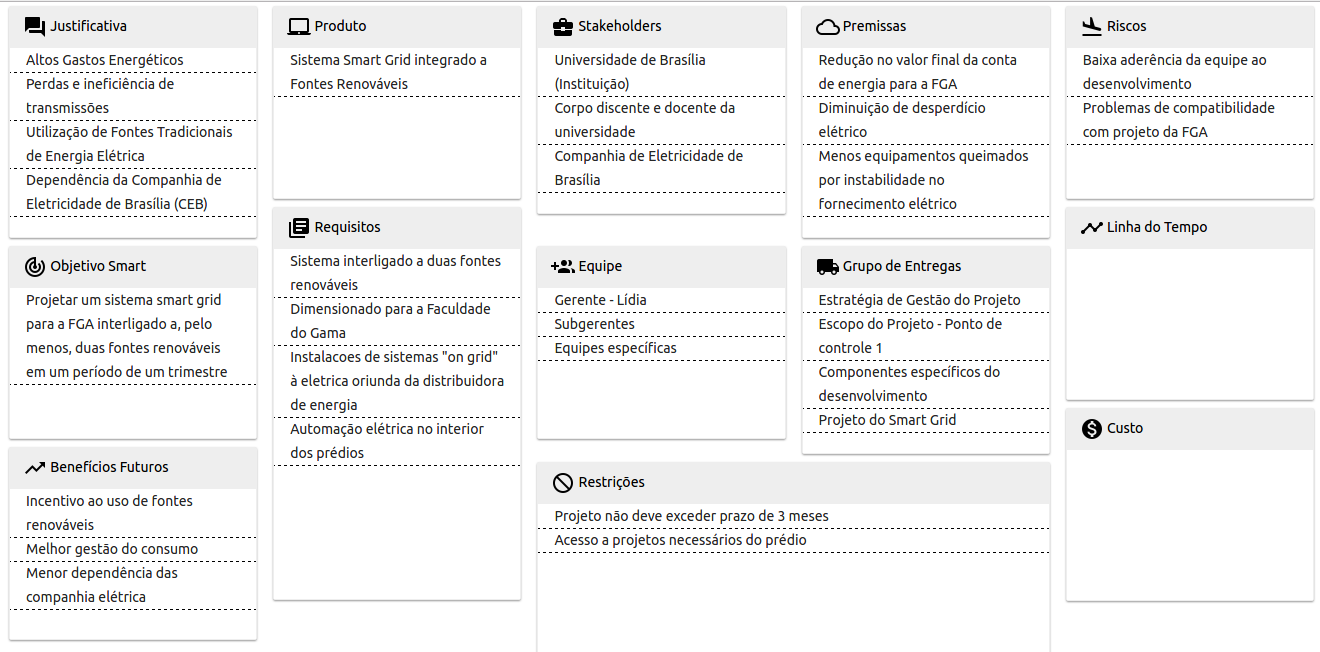
\includegraphics[width=0.75\paperwidth]{figuras/canvas.png}
\caption{Quadro do Canvas}
%\label{Rotulo}
\end{figure}